In this part, we introduce an approach of meta reinforcement learning for solving the problem of exploration, which is named model agnostic exploration with structured noise(MAESN). With the method an agent can be enabled to explore more effectively in new situations based on prior experience.
\subsection{overview}
It is well-known that exploration is a critical task in reinforcement learning. As the practical tasks are becoming more and more complex, the prior proposed exploration strategies such as information gain or state visitation bonuses perform not as well as expected, especially for multi-task problems. The approach model agnostic exploration with structured noise (MAESN), that has a combination of structured stochasticity with MAML, offers exploration strategies that are informed by prior knowledges and are more effective than random action-space noise.

The core idea of this gradient-based algorithm is to use prior experience both to initialize a policy and to learn a latent exploration space, by which the structured stochasticity injected policy can produce more effective exploration strategies on new task.

\subsection{ Meta-Learning Latent Variable Policies}
The conventional action distribution in reinforcement learning is written as $\pi_{\theta}(a\mid s)$, which possesses no property of temporally coherent randomness throughout the trajectory because it is independent for each time step. TO address this problem we introduce latent variables $Z$. 
\begin{figure}[H]
	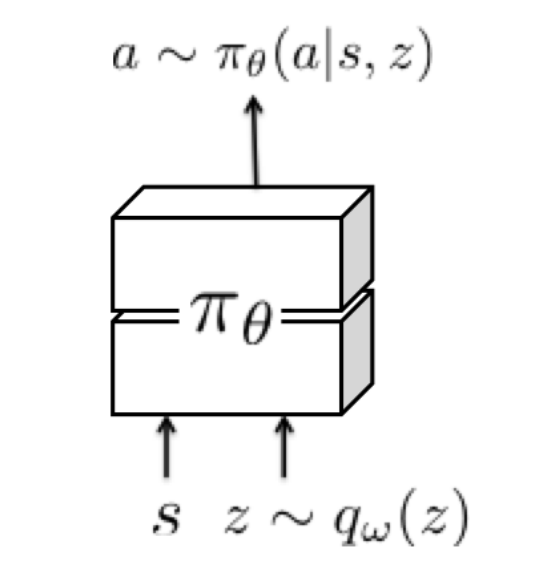
\includegraphics[scale=0.6]{MAESN_01.PNG}
	\centering
	\caption{latent variables}
	\label{MAESN}
\end{figure}

 We condition the policy on random variables, which are randomly drawn from a learned latent distribution. As the latent variable is sampled once per episode, the structured stochasticity in the process of exploration can be certainly ensured. The latent variable conditioned policy is represented as $\pi_{\theta}(a \mid s, z)$, where $z \sim q_{\omega}(z)$ and $q_{\omega}(z)$ is latent variable distribution with parameter $w$. 

Our aim is to meta-train the latent variable conditioned policy to generate coherent exploration strategies that perform faster adaptation on new tasks. Briefly, we jointly learn a set of policy parameters $\theta$ and the parameters of latent space distribution $w$, such that a policy gradient adaptation step can lead to maximal rewards.

\begin{figure}[H]
	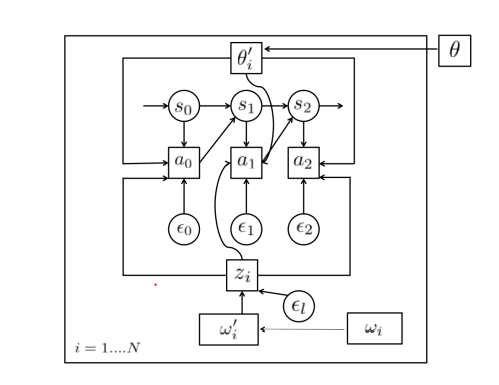
\includegraphics[scale=0.7]{MAESN_02.PNG}
	\centering
	\caption{Computation graph for MAESN}
	\label{MAESN}
\end{figure}

The objective of meta-training consists of not only sum of rewards through the whole trajectory, but also the KL-divergence between the per-task pre-update distributions $q_{\omega_{i}}\left(z_{i}\right)$ and a prior $p(z)$, which is usually a unit Gaussian, because the KL-divergence ensures a effective structured exploration.
The full meta-training problem can be stated mathematically as:

\begin{figure}[H]
	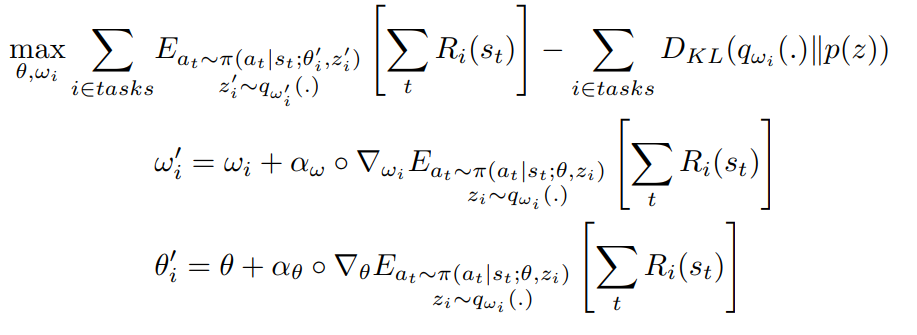
\includegraphics[scale=0.48]{MAESN_03.PNG}
	\centering
	\caption{meta-training procedure}
	\label{MAESN}
\end{figure}













